\section{Preventivo}
La suddivisione oraria viene fatta tenendo conto del fatto che nel corso del progetto ogni  membro del gruppo deve ricoprire ogni ruolo almeno una volta.
Per facilitare la lettura delle successive tabelle sono state utilizzate le seguenti abbreviazioni per identificare i diversi ruoli:
\begin{itemize}
	\item \textbf{Re}: \textit{Responsabile};
	\item \textbf{Am}: \textit{Amministratore};
	\item \textbf{An}: \textit{Analista};
	\item \textbf{Pt}: \textit{Progettista};
	\item \textbf{Pm}: \textit{Programmatore};
	\item \textbf{Ve}: \textit{Verificatore};
\end{itemize}
Inoltre per determinare le ore nulle nelle successive tabelle verrà usato il simbolo -, che ne indica l'assenza.

\subsection{Fase di Analisi}
\subsubsection{Prospetto orario}
Nella fase di Analisi la distribuzione oraria è la seguente:
\begin{table}[H]
	\rowcolors{2}{lightest-grayest}{white}
	\centering
	\renewcommand{\arraystretch}{1.5}
	\begin{tabular}{|c|c|c|c|c|c|c|c|}
		\hline
		\rowcolor{lighter-grayer}
		Nome & Re & Am & An & Pt & Pm & Ve & Totale\\
		\hline
		
		% ----- Modificare da qui -----
		%  collegamento tabella a indice tabelle, dati;
Badan Antonio     & - & - & 20 & - & - & 16 & 36  \\ \hline
Bertoldo Damiano  & - & 20 & - & - & - & 16 & 36  \\ \hline
Budai Matteo      & 10 & - & 20 & - & - & 6  & 36  \\ \hline
De Grandi Samuele & 10 & - & 20 & - & - & 6  & 36  \\ \hline
Piacere Ivan      & 10 & - & 20 & - & - & 6  & 36  \\ \hline
Privitera Sara    & - & 20 & - & - & - & 16 & 36  \\ \hline
Spigolon Daniele  & - & 20 & - & - & - & 16 & 36  \\ \hline
\textbf{Totale}   & 30 & 60 & 80 & - & - & 82 & 252 \\ \hline
		
\end{tabular}
\caption*{\textbf{Tabella 2}: Distribuzione delle ore nella Fase di Analisi\\}
\end{table}	

I dati ottenuti possono essere riassunti nel seguente istogramma:
% fare istogramma (con dati poi), collegare all'indice delle figure;
\begin{figure}[H]
	\centering
	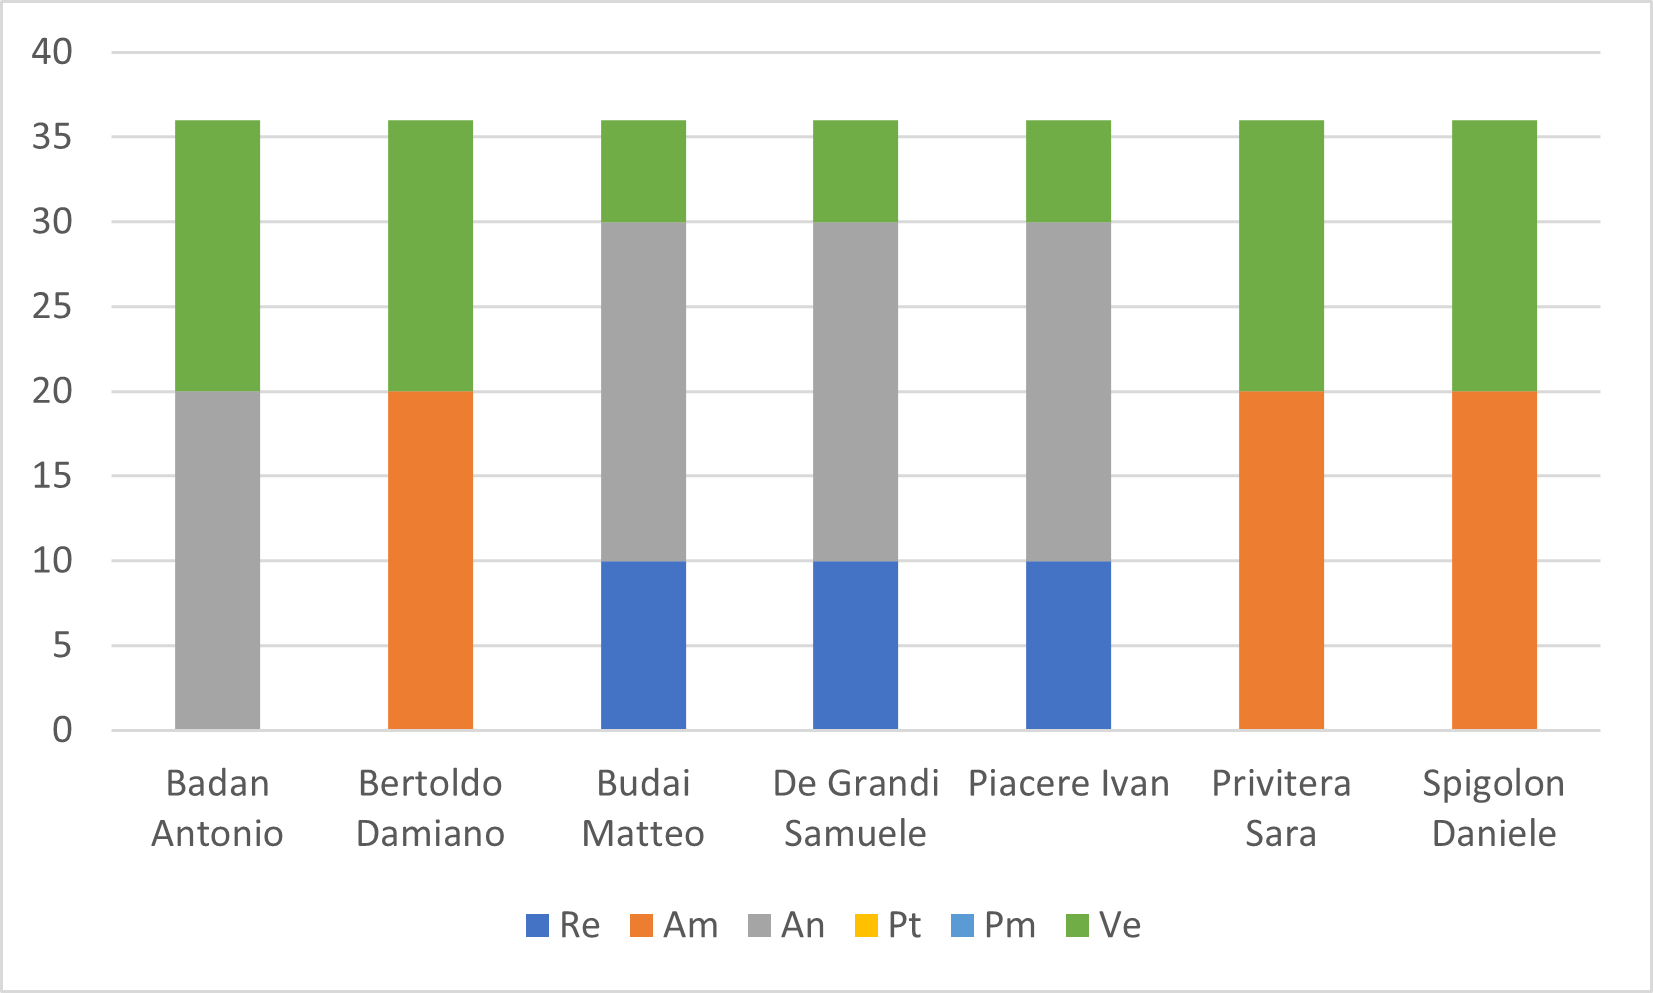
\includegraphics[width=0.7\linewidth]{res/images/Figura2.png}
	\caption*{\textbf{Figura2}: Istogramma della suddivisione delle ore durante la Fase di Analisi}
	\label{fig:Figura2}
\end{figure}

\subsubsection{Prospetto economico}
In questa fase il costo per ogni ruolo è il seguente:

\begin{table}[H]
	\rowcolors{2}{lightest-grayest}{white}
	\centering
	\renewcommand{\arraystretch}{1.5}
	\begin{tabular}{|c|c|c|}
		\hline
		\rowcolor{lighter-grayer}
		Ruolo & Ore & Costo\\
Responsabile  & 30  & 900  \\ \hline
Amministatore & 60  & 1320 \\ \hline
Analista      & 80  & 2000 \\ \hline
Progettista   & - & - \\ \hline
Programmatore & - & - \\ \hline
Verificatore  & 82  & 1312 \\ \hline
\textbf{Totale}& 252 & 5532 \\ \hline
\end{tabular}
	\caption*{\textbf{Tabella 3}: Prospetto dei costi per ruolo nella Fase di Analisi\\}
\end{table}
I dati ottenuti possono essere riassunti nel seguente areogramma:
%collegare all'indice delle figure;
\begin{figure}[H]
	\centering
	\begin{tikzpicture}
		\pie{11.9/Responsabile, 23.8/Amministartore, 31.7/Analista, 32.5/Verificatore}
	\end{tikzpicture}
	\caption*{\textbf{Figura 3}:  Areogramma della ripartizione di ore per ruolo nella Fase di Analisi}
	\label{fig:Figura3}
\end{figure}	



\subsection{Fase di Progettazione architetturale}
\subsubsection{Prospetto orario}
Nella fase di Progettazione architetturale la distribuzione oraria è la seguente:

\begin{table}[H]
	\rowcolors{2}{lightest-grayest}{white}
	\centering
	\renewcommand{\arraystretch}{1.5}
	\begin{tabular}{|c|c|c|c|c|c|c|c|}
		\hline
		\rowcolor{lighter-grayer}
		Nome & Re & Am & An & Pt & Pm & Ve & Totale ore\\
Badan Antonio     & 3  & 1  & 5  & 9  & - & 5  & 23  \\ \hline
Bertoldo Damiano  & 3  & 1  & 5  & 9  & - & 5  & 23  \\ \hline
Budai Matteo      & - & 1  & 6  & 10 & - & 6  & 23  \\ \hline
De Grandi Samuele & - & 1  & 6  & 10 & - & 6  & 23  \\ \hline
Piacere Ivan      & - & 2  & 6  & 9  & - & 6  & 23  \\ \hline
Privitera Sara    & 2  & 2  & 6  & 7  & - & 6  & 23  \\ \hline
Spigolon Daniele  & 2  & 2  & 6  & 7  & - & 6  & 23  \\ \hline
\textbf{Totale}   & 10 & 10 & 40 & 61 & - & 40 & 161 \\ \hline
	\end{tabular}
	\caption*{\textbf{Tabella 4}: Distribuzione delle ore nel periodo di Progettazione architetturale\\}
\end{table}	
I dati ottenuti possono essere riassunti nel seguente istogramma:

\begin{figure}[H]
	\centering
	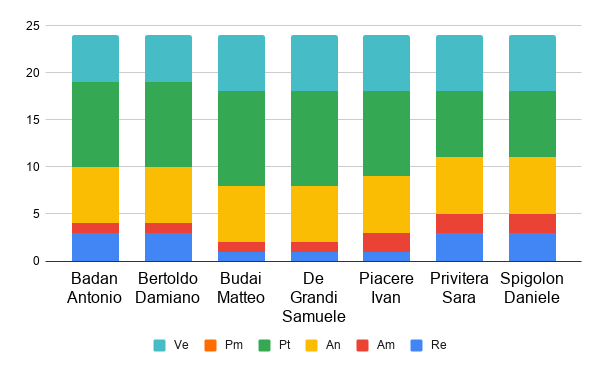
\includegraphics[width=0.7\linewidth]{res/images/IstogrammaFase2.png}
	\caption*{\textbf{Figura 4}: Istogramma della suddivisione delle ore durante il periodo di Progettazione architetturale}
	\label{fig:Figura10}
\end{figure}


\subsubsection{Prospetto economico}
In questa fase il costo per ogni ruolo è il seguente:

\begin{table}[H]
	\rowcolors{2}{lightest-grayest}{white}
	\centering
	\renewcommand{\arraystretch}{1.5}
	\begin{tabular}{|c|c|c|}
		\hline
		\rowcolor{lighter-grayer}
		Ruolo & Ore & Costo \\
Responsabile   & 10  & 300  \\ \hline
Amministratore & 10  & 220  \\ \hline
Analista       & 40  & 1000 \\ \hline
Progettista    & 61  & 1464 \\ \hline
Programmatore  & - & - \\ \hline
Verificatore   & 40  & 640  \\ \hline
\textbf{Totale}& 161 & 3624 \\ \hline
	\end{tabular}
	\caption*{\textbf{Tabella 5}: Prospetto dei costi per ruolo nel periodo di Progettazione architetturale\\}
\end{table}

I dati ottenuti possono essere riassunti nel seguente areogramma:


\begin{figure}[H]
	\centering
	\begin{tikzpicture}
		\pie{6.2/Responsabile, 6.2/Amministratore, 24.8/Analista, 37.9/Progettista, 24.8/Verificatore}
	\end{tikzpicture}
	\caption*{\textbf{Figura 5}: Areogramma della ripartizione di ore per ruolo in Progettazione architetturale}
	\label{fig:Figura10}
\end{figure}



\subsection{Fase di Progettazione di dettaglio e codifica}
\subsubsection{Prospetto orario}
Nella fase di Progettazione di dettaglio e codifica la distribuzione oraria è la seguente:

\begin{table}[H]
	\rowcolors{2}{lightest-grayest}{white}
	\centering
	\renewcommand{\arraystretch}{1.5}
	\begin{tabular}{|c|c|c|c|c|c|c|c|}
		\hline
		\rowcolor{lighter-grayer}
		Nome & Re & Am & An & Pt & Pm & Ve & Totale ore\\
Badan Antonio     & 4  & 5  & 4  & 3  & 20  & 14  & 50  \\ \hline
Bertoldo Damiano  & 4  & 5  & 4  & - & 20  & 17  & 50  \\ \hline
Budai Matteo      & 5  & 6  & 4  & 5  & 20  & 10  & 50  \\ \hline
De Grandi Samuele & 4  & 6  & - & 5  & 20  & 15  & 50  \\ \hline
Piacere Ivan      & 5  & 6  & - & 5  & 20  & 14  & 50  \\ \hline
Privitera Sara    & 4  & 6  & 3  & - & 19  & 18  & 50  \\ \hline
Spigolon Daniele  & 4  & 6  & 5  & 2  & 21  & 12  & 50  \\ \hline
\textbf{Totale}   & 30 & 40 & 20 & 20 & 140 & 100 & 350 \\ \hline
	\end{tabular}
	\caption*{\textbf{Tabella 6}: Distribuzione delle ore nel periodo di Progettazione di dettaglio e codifica\\}
\end{table}	
I dati ottenuti possono essere riassunti nel seguente istogramma:

\begin{figure}[H]
	\centering
	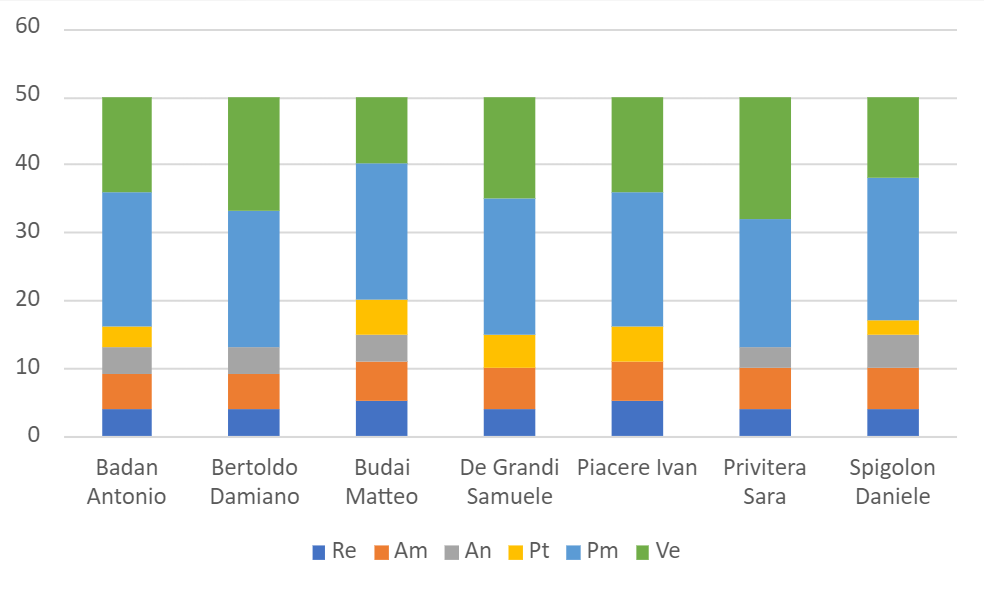
\includegraphics[width=0.7\linewidth]{res/images/IstogrammaFase3.png}
	\caption*{\textbf{Figura 6}: Istogramma della suddivisione delle ore durante il periodo di Progettazione di dettaglio e codifica}
	\label{fig:Figura10}
\end{figure}


\subsubsection{Prospetto economico}
In questa fase il costo per ogni ruolo è il seguente:

\begin{table}[H]
	\rowcolors{2}{lightest-grayest}{white}
	\centering
	\renewcommand{\arraystretch}{1.5}
	\begin{tabular}{|c|c|c|}
		\hline
		\rowcolor{lighter-grayer}
		Ruolo & Ore & Costo \\
Responsabile   & 30  & 900  \\ \hline
Amministratore & 40  & 880  \\ \hline
Analista       & 20  & 500  \\ \hline
Progettista    & 20  & 480  \\ \hline
Programmatore  & 140 & 2240 \\ \hline
Verificatore   & 100 & 1600 \\ \hline
\textbf{Totale}& 350 & 6600 \\ \hline
	\end{tabular}
	\caption*{\textbf{Tabella 7}: Prospetto dei costi per ruolo nel periodo di Progettazione di dettaglio e codifica\\}
\end{table}

I dati ottenuti possono essere riassunti nel seguente areogramma:


\begin{figure}[H]
	\centering
	\begin{tikzpicture}
		\pie{8.6/Responsabile, 11.4/Amministratore, 5.7/Analista, 5.7/Progettista, 40/Programmatore, 28.6/Verificatore}
	\end{tikzpicture}
	\caption*{\textbf{Figura 8}: Areogramma della ripartizione di ore per ruolo in Progettazione di dettaglio e codifica}
	\label{fig:Figura10}
\end{figure}

\subsection{Fase di Validazione e collaudo}
\subsubsection{Prospetto orario}
Nella fase di Validazione e collaudo la distribuzione oraria è la seguente:

\begin{table}[H]
	\rowcolors{2}{lightest-grayest}{white}
	\centering
	\renewcommand{\arraystretch}{1.5}
	\begin{tabular}{|c|c|c|c|c|c|c|c|}
		\hline
		\rowcolor{lighter-grayer}
		Nome & Re & Am & An & Pt & Pm & Ve & Totale ore\\
Badan Antonio     & 4  & - & - & 10 & 4  & 7  & 25  \\ \hline
Bertoldo Damiano  & 6  & - & - & - & 10 & 9  & 25  \\ \hline
Budai Matteo      & - & 9  & - & - & 5  & 11 & 25  \\ \hline
De Grandi Samuele & - & 7  & - & 5  & 4  & 9  & 25  \\ \hline
Piacere Ivan      & - & 8  & - & - & 4  & 13 & 25  \\ \hline
Privitera Sara    & 6  & - & - & 10 & 6  & 3  & 25  \\ \hline
Spigolon Daniele  & 4  & - & - & - & 10 & 11 & 25  \\ \hline
\textbf{Totale}   & 20 & 24 & - & 25 & 43 & 63 & 175 \\ \hline
	\end{tabular}
	\caption*{\textbf{Tabella 9}: Distribuzione delle ore nel periodo di Validazione e collaudo\\}
\end{table}	
	I dati ottenuti possono essere riassunti nel seguente istogramma:

\begin{figure}[H]
	\centering
	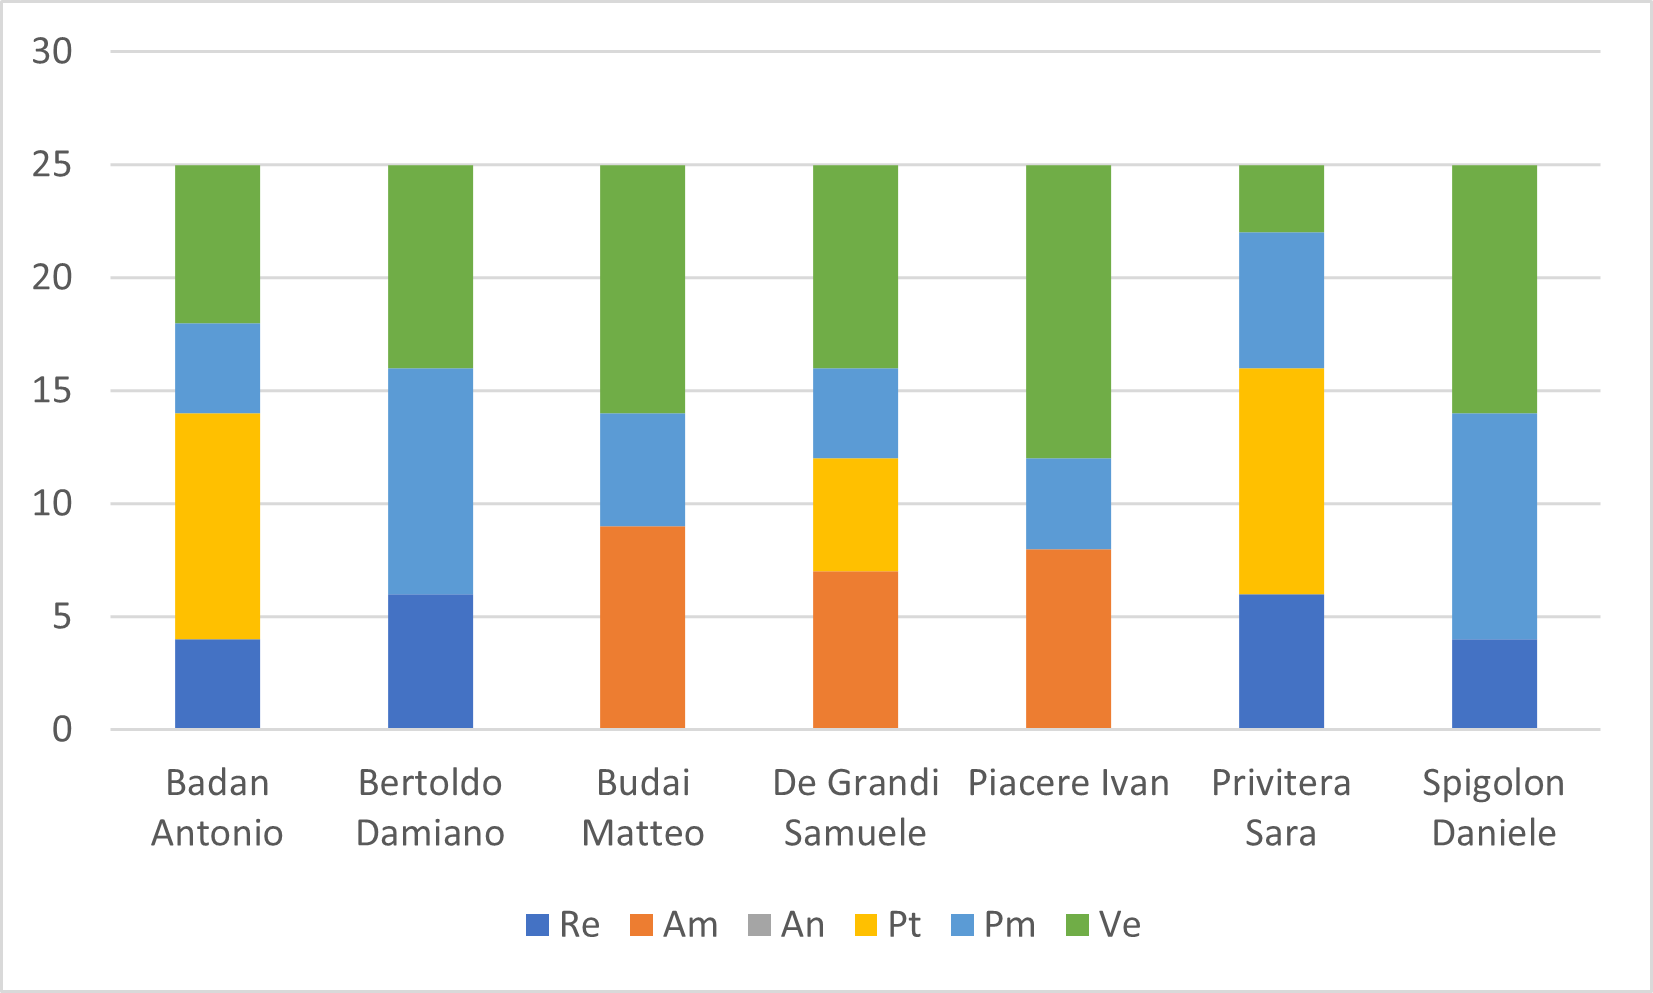
\includegraphics[width=0.7\linewidth]{res/images/Figura11.png}
	\caption*{\textbf{Figura 9}: Istogramma della suddivisione delle ore durante il periodo di Validazione e collaudo}
	\label{fig:Figura10}
\end{figure}
	
	
\subsubsection{Prospetto economico}
In questa fase il costo per ogni ruolo è il seguente:

\begin{table}[H]
	\rowcolors{2}{lightest-grayest}{white}
	\centering
	\renewcommand{\arraystretch}{1.5}
	\begin{tabular}{|c|c|c|}
		\hline
		\rowcolor{lighter-grayer}
		Ruolo & Ore & Costo \\
Responsabile   & 20  & 600  \\ \hline
Amministratore & 24  & 528  \\ \hline
Analista       & - & - \\ \hline
Progettista    & 25  & 600  \\ \hline
Programmatore  & 43  & 688  \\ \hline
Verificatore   & 63  & 1008 \\ \hline
\textbf{Totale}& 175 & 3424 \\ \hline
	\end{tabular}
\caption*{\textbf{Tabella 10}: Prospetto dei costi per ruolo nel periodo di Validazione e collaudo\\}
\end{table}

I dati ottenuti possono essere riassunti nel seguente areogramma:


\begin{figure}[H]
	\centering
	\begin{tikzpicture}
		\pie{11.4/Responsabile, 13.7/Amministratore, 14.3/Progettista, 24.6/Programmatore,  36/Verificatore}
	\end{tikzpicture}
	\caption*{\textbf{Figura 10}: Areogramma della ripartizione di ore per ruolo in Validazione e collaudo}
	\label{fig:Figura10}
\end{figure}

\subsection{Riepilogo}
\subsubsection{Ore totali}
\paragraph{Prospetto orario totale}
Nella seguente tabella viene riportata la distribuzione oraria di tutte le fasi:

\begin{table}[H]
	\rowcolors{2}{lightest-grayest}{white}
	\centering
	\renewcommand{\arraystretch}{1.5}
	\begin{tabular}{|c|c|c|c|c|c|c|c|}
		\hline
		\rowcolor{lighter-grayer}
		Nome & Re & Am & An & Pt & Pm & Ve & Totale ore\\
Badan Antonio     & 11 & 6   & 29  & 22  & 24  & 42  & 134 \\ \hline
Bertoldo Damiano  & 13 & 26  & 9   & 9   & 30  & 47  & 134 \\ \hline
Budai Matteo      & 15 & 16  & 30  & 15  & 25  & 33  & 134 \\ \hline
De Grandi Samuele & 14 & 14  & 26  & 20  & 24  & 36  & 134 \\ \hline
Piacere Ivan      & 15 & 16  & 26  & 14  & 24  & 39  & 134 \\ \hline
Privitera Sara    & 12 & 28  & 9   & 17  & 25  & 43  & 134 \\ \hline
Spigolon Daniele  & 10 & 28  & 11  & 9   & 31  & 45  & 134 \\ \hline
\textbf{Totale}   & 90 & 134 & 140 & 106 & 183 & 285 & 938 \\ \hline
	\end{tabular}
	\caption*{\textbf{Tabella 11}: Prospetto orario che comprende tutte le fasi trattate in precedenza\\}
\end{table}	
I dati ottenuti possono essere riassunti nel seguente istogramma:

\begin{figure}[H]
	\centering
	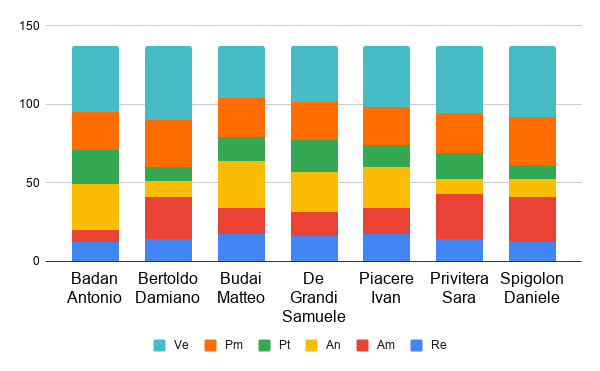
\includegraphics[width=0.7\linewidth]{res/images/IstogrammaTotale.png}
	\caption*{\textbf{Figura11}: Istogramma della suddivisione delle ore di tutte le fasi trattate in precedenza}
	\label{fig:Figura10}
\end{figure}

\paragraph{Prospetto economico totale}
Nella seguente tabella vengono mostrati i costi complessivi per ogni ruolo:

\begin{table}[H]
	\rowcolors{2}{lightest-grayest}{white}
	\centering
	\renewcommand{\arraystretch}{1.5}
	\begin{tabular}{|c|c|c|}
		\hline
		\rowcolor{lighter-grayer}
		Ruolo & Ore & Costo \\
Responsabile   & 90  & 2700  \\ \hline
Amministratore & 134 & 2948  \\ \hline
Analista       & 140 & 3500  \\ \hline
Progettista    & 106 & 2544  \\ \hline
Programmatore  & 183 & 2928  \\ \hline
Verificatore   & 285 & 4560  \\ \hline
\textbf{Totale}& 938 & 19180 \\ \hline
	\end{tabular}
	\caption*{\textbf{Tabella 12}: Prospetto dei costi totali per ciascun ruolo \\}
\end{table}

I dati ottenuti possono essere riassunti nel seguente areogramma:


\begin{figure}[H]
	\centering
	\begin{tikzpicture}
		\pie{9.6/Responsabile, 14.3/Amministratore, 14.9/Analista, 11.3/Progettista, 19.5/Programmatore,  30.4/Verificatore}
	\end{tikzpicture}
	\caption*{\textbf{Figura 12}: Areogramma dei costi totali delle ore di investimento e rendicontate}
    \label{fig:Figura10}
\end{figure}

\subsubsection{Ore totali rendicontate}
\paragraph{Prospetto orario totale rendicontato}
Nella seguente tabella viene riportata la distribuzione oraria di tutte le fasi a carico del committente, ad esclusione quindi, dell'Analisi e del Consolidamento dei requisiti:

\begin{table}[H]
	\rowcolors{2}{lightest-grayest}{white}
	\centering
	\renewcommand{\arraystretch}{1.5}
	\begin{tabular}{|c|c|c|c|c|c|c|c|}
		\hline
		\rowcolor{lighter-grayer}
		Nome & Re & Am & An & Pt & Pm & Ve & Totale ore\\
Badan Antonio     & 11 & 6  & 9  & 22  & 24  & 26  & 98  \\ \hline
Bertoldo Damiano  & 13 & 6  & 9  & 9   & 30  & 31  & 98  \\ \hline
Budai Matteo      & 5  & 16 & 10 & 15  & 25  & 27  & 98  \\ \hline
De Grandi Samuele & 4  & 14 & 6  & 20  & 24  & 30  & 98  \\ \hline
Piacere Ivan      & 5  & 16 & 6  & 14  & 24  & 33  & 98  \\ \hline
Privitera Sara    & 12 & 8  & 9  & 17  & 25  & 27  & 98  \\ \hline
Spigolon Daniele  & 10 & 8  & 11 & 9   & 31  & 29  & 98  \\ \hline
\textbf{Totale}   & 60 & 74 & 60 & 106 & 183 & 203 & 686 \\ \hline
	\end{tabular}
	\caption*{\textbf{Tabella 13}: Prospetto orario che comprende tutte le ore rendicontate\\}
\end{table}	
I dati ottenuti possono essere riassunti nel seguente istogramma:

\begin{figure}[H]
	\centering
	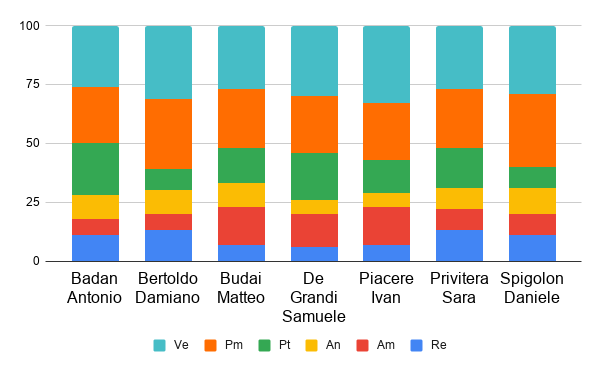
\includegraphics[width=0.7\linewidth]{res/images/IstogrammaTotaleRendicontato.png}
	\caption*{\textbf{Figura 13}: Istogramma della suddivisione delle ore rendicontate}
	\label{fig:Figura10}
\end{figure}

\paragraph{Prospetto economico totale rendicontato}
Nella seguente tabella vengono mostrati i costi complessivi rendicontati per ogni ruolo:

\begin{table}[H]
	\rowcolors{2}{lightest-grayest}{white}
	\centering
	\renewcommand{\arraystretch}{1.5}
	\begin{tabular}{|c|c|c|}
		\hline
		\rowcolor{lighter-grayer}
		Ruolo & Ore & Costo \\
Responsabile   & 60  & 1800  \\ \hline
Amministratore & 74  & 1628  \\ \hline
Analista       & 60  & 1500  \\ \hline
Progettista    & 106 & 2544  \\ \hline
Programmatore  & 183 & 2928  \\ \hline
Verificatore   & 203 & 3248  \\ \hline
\textbf{Totale}& 686 & 13648 \\ \hline
	\end{tabular}
	\caption*{\textbf{Tabella 14}: Prospetto dei costi totali rendicontati \\}
\end{table}

I dati ottenuti possono essere riassunti nel seguente areogramma:


\begin{figure}[H]
	\centering
	\begin{tikzpicture}
		\pie{8.7/Responsabile, 10.8/Amministratore, 8.7/Analista, 15.5/Progettista, 26.7/Programmatore, 29.6/Verificatore}
	\end{tikzpicture}
	\caption*{\textbf{Figura 14}: Areogramma delle ore rendicontate per ruolo}
    \label{fig:Figura10}
\end{figure}

\subsubsection{Conclusioni}
Il costo del progetto considerando le ore rendicontate è: 13648\euro.